
\documentclass[ review  , 3p ]{elsarticle}
%default = preprint (single sapce), review = doublespace
%detail class option: https://www.elsevier.com/__data/assets/pdf_file/0008/56843/elsdoc-1.pdf

% eliminate "Preprinted to Elsevier"
\makeatletter
\def\ps@pprintTitle{%
 \let\@oddhead\@empty
 \let\@evenhead\@empty
 \def\@oddfoot{\centerline{\thepage}}%
 \let\@evenfoot\@oddfoot}
\makeatother

%%% Begin My package additions %%%%%%%%%%%%%%%%%%%
\usepackage[hyphens]{url}



\usepackage{lineno} % add
\providecommand{\tightlist}{%
  \setlength{\itemsep}{0pt}\setlength{\parskip}{0pt}}

\usepackage{graphicx}

\usepackage{zxjatype}
\usepackage{xeCJK}
\setCJKmainfont{ipaexm.ttf}
\setCJKsansfont{ipaexg.ttf}
\setCJKmonofont{ipaexg.ttf}

\usepackage{color}

\usepackage{booktabs}
\usepackage{longtable}
\usepackage{array}
\usepackage{multirow}
\usepackage{wrapfig}
\usepackage{float}
\usepackage{colortbl}
\usepackage{pdflscape}
\usepackage{tabu}
\usepackage{threeparttable}
\usepackage{threeparttablex}
\usepackage[normalem]{ulem}
\usepackage{makecell}
\usepackage{xcolor}


%\usepackage{xpatch}
%\xpatchcmd{\MaketitleBox}{\hrule}{}{}{}% remove first horizontal rule (above abstract)
%\xpatchcmd{\MaketitleBox}{\hrule}{}{}{}% remoce second horizonral rule (below keywords)
%%%%%%%%%%%%%%%% end my additions to header

\usepackage[T1]{fontenc}
\usepackage{lmodern}
\usepackage{amssymb,amsmath}
\usepackage{ifxetex,ifluatex}
\usepackage{fixltx2e} % provides \textsubscript
% use upquote if available, for straight quotes in verbatim environments
\IfFileExists{upquote.sty}{\usepackage{upquote}}{}
\ifnum 0\ifxetex 1\fi\ifluatex 1\fi=0 % if pdftex
  \usepackage[utf8]{inputenc}
\else % if luatex or xelatex
  \usepackage{fontspec}
  \ifxetex
    \usepackage{xltxtra,xunicode}
  \fi
  \defaultfontfeatures{Mapping=tex-text,Scale=MatchLowercase}
  \newcommand{\euro}{€}
\fi
% use microtype if available
\IfFileExists{microtype.sty}{\usepackage{microtype}}{}
\bibliographystyle{elsarticle-harvard}
\usepackage{tabularx}
\ifxetex
  \usepackage[setpagesize=false, % page size defined by xetex
              unicode=false, % unicode breaks when used with xetex
              xetex]{hyperref}
\else
  \usepackage[unicode=true]{hyperref}
\fi
\hypersetup{breaklinks=true,
            bookmarks=true,
            pdfauthor={},
            pdftitle={Short Paper},
            colorlinks=false,
            urlcolor=blue,
            linkcolor=magenta,
            pdfborder={0 0 0}}
\urlstyle{same}  % don't use monospace font for urls

\setcounter{secnumdepth}{5}

\newlength{\cslhangindent}
\setlength{\cslhangindent}{1.5em}
\newlength{\csllabelwidth}
\setlength{\csllabelwidth}{3em}
\newenvironment{CSLReferences}[3] % #1 hanging-ident, #2 entry spacing
 {% don't indent paragraphs
  \setlength{\parindent}{0pt}
  % turn on hanging indent if param 1 is 1
  \ifodd #1 \everypar{\setlength{\hangindent}{\cslhangindent}}\ignorespaces\fi
  % set entry spacing
  \ifnum #2 > 0
  \setlength{\parskip}{#2\baselineskip}
  \fi
 }%
 {}
\usepackage{calc} % for \widthof, \maxof
\newcommand{\CSLBlock}[1]{#1\hfill\break}
\newcommand{\CSLLeftMargin}[1]{\parbox[t]{\maxof{\widthof{#1}}{\csllabelwidth}}{#1}}
\newcommand{\CSLRightInline}[1]{\parbox[t]{\linewidth}{#1}}
\newcommand{\CSLIndent}[1]{\hspace{\cslhangindent}#1}

% Pandoc toggle for numbering sections (defaults to be off)


% Pandoc header


\begin{document}
  \begin{frontmatter}

    \title{Charitable Giving, Tax Reform, and Government Efficiency\tnoteref{1}}
            \tnotetext[1]{This research is base on}
                \author[Osaka University]{
      Hiroki Kato 
       \corref{*} }
     \ead{vge008kh@stundent.econ.osaka-u.ac.jp}   %to avoid auto-link, use \@ instead of @
        \author[Chiba University]{
      Tsuyoshi Goto 
      }
      %to avoid auto-link, use \@ instead of @
        \author[Kobe University]{
      Yong-Rok Kim 
      }
      %to avoid auto-link, use \@ instead of @
            \address[Osaka University]{Graduate School of Economics, Osaka University, Japan}
        \address[Chiba University]{Graduate School of Economics, Chiba University, Japan}
        \address[Kobe University]{Graduate School of Economics, Kobe University, Japan}
            \cortext[*]{Corresponding Author.}
      
        \begin{abstract}
      Brah
    \end{abstract}
      
        \begin{keyword}
      Charitable giving, Giving price, Tax reform, Governement efficiency, South Korea
       \JEL{D91, I10, I18} 
    \end{keyword}
    
  \end{frontmatter}

  \hypertarget{introduction}{%
  \section{Introduction}\label{introduction}}
  
  Placeholder
  
  \hypertarget{charitable-giving-and-taxiation}{%
  \subsection{Charitable Giving and Taxiation}\label{charitable-giving-and-taxiation}}
  
  \hypertarget{summary-in-short}{%
  \subsection{Summary in short}\label{summary-in-short}}
  
  \hypertarget{south-korean-tax-reform}{%
  \subsection{South Korean tax reform}\label{south-korean-tax-reform}}
  
  \hypertarget{related-literature}{%
  \subsection{Related Literature}\label{related-literature}}
  
  \hypertarget{research-about-tax-price-elasticity-of-charitable-donations}{%
  \subsection{Research about tax price elasticity of charitable donations}\label{research-about-tax-price-elasticity-of-charitable-donations}}
  
  \hypertarget{research-about-perception-towards-the-government-and-donationtax-payment.}{%
  \subsection{Research about perception towards the government and donation/tax payment.}\label{research-about-perception-towards-the-government-and-donationtax-payment.}}
  
  \hypertarget{why-political-trust}{%
  \subsection{Why Political Trust?}\label{why-political-trust}}
  
  \hypertarget{institutional-background}{%
  \section{Institutional background}\label{institutional-background}}
  
  Placeholder
  
  \hypertarget{tax-relief-for-charitable-giving-by-tax-deduction-and-tax-credit}{%
  \subsection{Tax relief for charitable giving by tax deduction and tax credit}\label{tax-relief-for-charitable-giving-by-tax-deduction-and-tax-credit}}
  
  \hypertarget{korean-tax-reform-in-2014-need-modification-by-kim-san}{%
  \subsection{Korean tax reform in 2014 (Need modification by Kim san)}\label{korean-tax-reform-in-2014-need-modification-by-kim-san}}
  
  \hypertarget{data}{%
  \section{Data}\label{data}}
  
  Placeholder
  
  \hypertarget{national-survey-of-tax-and-benefit-nastab}{%
  \subsection{National Survey of Tax and Benefit (NaSTaB)}\label{national-survey-of-tax-and-benefit-nastab}}
  
  \hypertarget{time-series-of-chariable-giving}{%
  \subsection{Time Series of Chariable Giving}\label{time-series-of-chariable-giving}}
  
  \hypertarget{summary-statistics}{%
  \subsection{Summary Statistics}\label{summary-statistics}}
  
  \hypertarget{what-is-giving-price}{%
  \subsection{What is Giving Price?}\label{what-is-giving-price}}
  
  \hypertarget{determination-of-tax-amount}{%
  \subsection{Determination of Tax Amount}\label{determination-of-tax-amount}}
  
  \hypertarget{derive-giving-price}{%
  \subsection{Derive Giving Price}\label{derive-giving-price}}
  
  \hypertarget{construct-giving-price}{%
  \subsection{Construct Giving Price}\label{construct-giving-price}}
  
  \hypertarget{income-distribution-and-giving-price}{%
  \subsection{Income Distribution and Giving Price}\label{income-distribution-and-giving-price}}
  
  \hypertarget{empirical-strategy}{%
  \subsection{Empirical Strategy}\label{empirical-strategy}}
  
  \hypertarget{intensive-margin-and-extensive-margin}{%
  \subsection{Intensive Margin and Extensive Margin}\label{intensive-margin-and-extensive-margin}}
  
  \hypertarget{main-results}{%
  \section{Main Results}\label{main-results}}
  
  \hypertarget{price-and-income-elasticity}{%
  \subsection{Price and Income Elasticity}\label{price-and-income-elasticity}}
  
  \begin{figure}
  
  {\centering 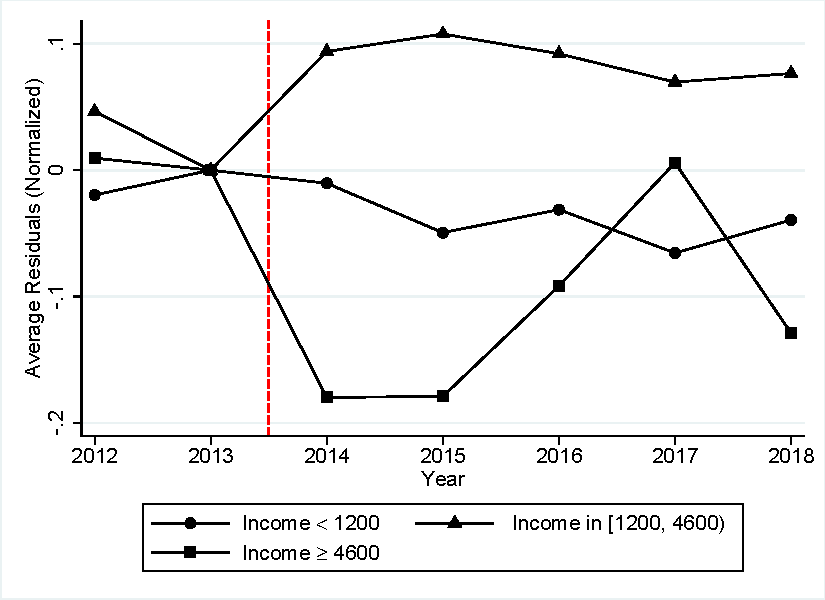
\includegraphics[width=0.9\linewidth]{C:/Users/vge00/Desktop/NaSTaB/_assets/ElasticityResid} 
  
  }
  
  \caption{Average Residuals Grouped by Year and Tax-Reform Benefit Group}\label{fig:unnamed-chunk-1}
  \end{figure}
  
  \begin{table}
  
  \caption{\label{tab:kableEstimateElasticityPart1}Main Results}
  \centering
  \fontsize{8}{10}\selectfont
  \begin{threeparttable}
  \begin{tabular}[t]{lccccc}
  \toprule
   & (1) & (2) & (3) & (4) & (5)\\
  \midrule
  ln(giving price) & -1.072*** & -1.264*** & -1.291*** & -1.114*** & -1.241***\\
   & (0.202) & (0.213) & (0.230) & (0.229) & (0.227)\\
  ln(auunaul taxable income) & 5.392*** & 5.080*** & 5.047*** & 5.116*** & 4.946***\\
   & (0.970) & (0.964) & (0.964) & (0.966) & (0.949)\\
  Individual FE & Y & Y & Y & Y & Y\\
  Time FE & Y & Y & Y & Y & Y\\
  Age & N & Y & Y & Y & Y\\
  Year X Education & N & N & Y & Y & Y\\
  Year X Gender & N & N & N & Y & Y\\
  Year X Resident Area & N & N & N & N & Y\\
  N & 53269 & 53269 & 53267 & 53267 & 53267\\
  R-sq & 0.009 & 0.010 & 0.010 & 0.011 & 0.020\\
  \bottomrule
  \end{tabular}
  \begin{tablenotes}
  \item Notes: $^{*}$ $p < 0.1$, $^{**}$ $p < 0.05$, $^{***}$ $p < 0.01$. Standard errors are clustered at individual level. When controlling age, we alson include its squared term.
  \end{tablenotes}
  \end{threeparttable}
  \end{table}
  
  \begin{figure}
  
  {\centering 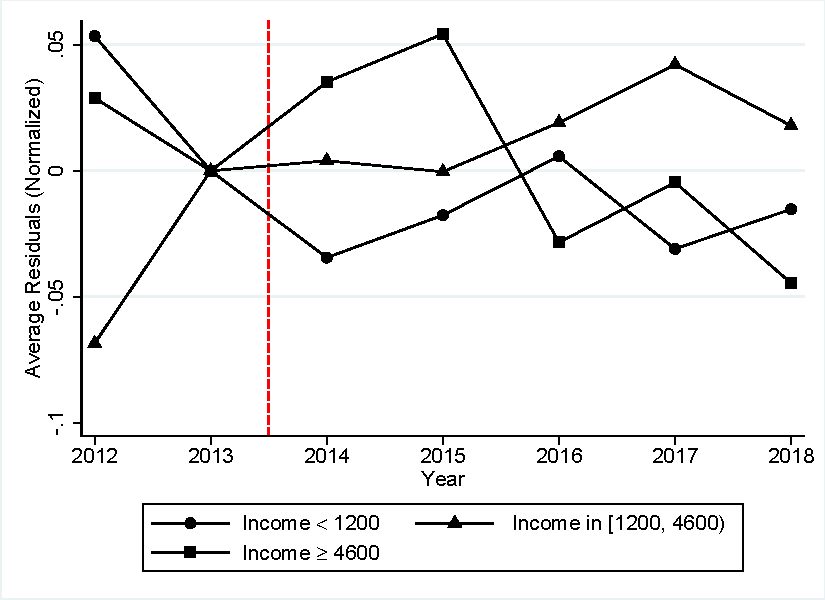
\includegraphics[width=0.9\linewidth]{C:/Users/vge00/Desktop/NaSTaB/_assets/IntElasticityResid} 
  
  }
  
  \caption{Average Residuals Grouped by Year and Tax-Reform Benefit Group (Intensive Margin)}\label{fig:unnamed-chunk-2}
  \end{figure}
  
  \begin{figure}
  
  {\centering 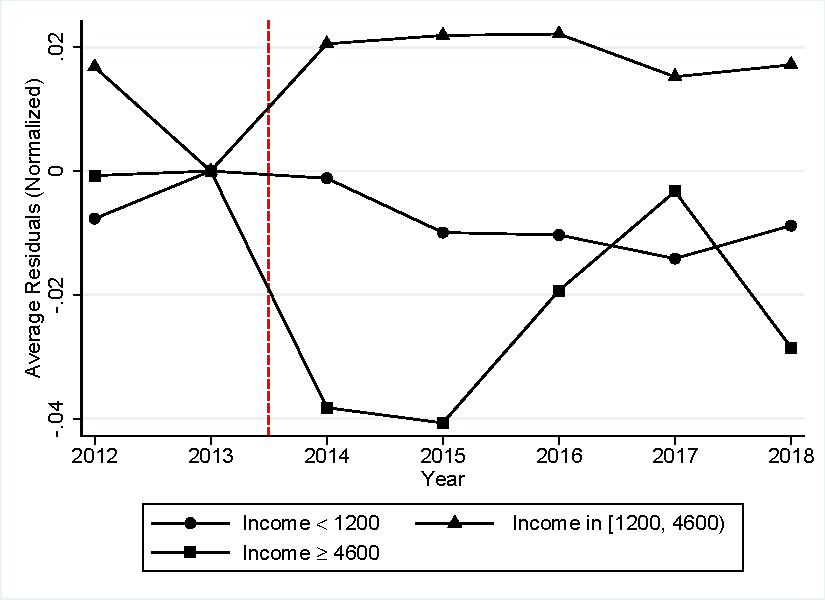
\includegraphics[width=0.9\linewidth]{C:/Users/vge00/Desktop/NaSTaB/_assets/ExtElasticityResid} 
  
  }
  
  \caption{Average Residuals Grouped by Year and Tax-Reform Benefit Group (Extensive Margin)}\label{fig:unnamed-chunk-3}
  \end{figure}
  
  \begin{table}
  
  \caption{\label{tab:kableEstimateElasticityPart2}Main Results: Intensive- and Extensive-Margin Elasticity}
  \centering
  \fontsize{8}{10}\selectfont
  \begin{threeparttable}
  \begin{tabular}[t]{lccccc}
  \toprule
   & (1) & (2) & (3) & (4) & (5)\\
  \midrule
  \addlinespace[0.3em]
  \multicolumn{6}{l}{\textbf{Intensive-Margin Elasticity}}\\
  \hspace{1em}ln(giving price) & -0.593*** & -0.838*** & -1.016*** & -0.893*** & -0.904***\\
  \hspace{1em} & (0.203) & (0.212) & (0.232) & (0.243) & (0.248)\\
  \hspace{1em}ln(auunaul taxable income) & 2.015*** & 1.562** & 1.445** & 1.528** & 1.571**\\
  \hspace{1em} & (0.675) & (0.655) & (0.647) & (0.651) & (0.653)\\
  \hspace{1em}N & 11637 & 11637 & 11637 & 11637 & 11637\\
  \hspace{1em}R-sq & 0.006 & 0.009 & 0.012 & 0.013 & 0.034\\
  \addlinespace[0.3em]
  \multicolumn{6}{l}{\textbf{Extensive-Margin Elasticity}}\\
  \hspace{1em}ln(giving price) & -0.257*** & -0.288*** & -0.273*** & -0.237*** & -0.267***\\
  \hspace{1em} & (0.046) & (0.048) & (0.052) & (0.052) & (0.051)\\
  \hspace{1em}ln(auunaul taxable income) & 1.175*** & 1.124*** & 1.125*** & 1.139*** & 1.102***\\
  \hspace{1em} & (0.223) & (0.223) & (0.223) & (0.224) & (0.220)\\
  \hspace{1em}Implied price elasiticity & -1.264*** & -1.418*** & -1.343*** & -1.167*** & -1.312***\\
  \hspace{1em} & (0.226) & (0.237) & (0.256) & (0.256) & (0.253)\\
  \hspace{1em}Implied income elasticity & 5.778*** & 5.527*** & 5.531*** & 5.600*** & 5.420***\\
  \hspace{1em} & (1.099) & (1.097) & (1.099) & (1.100) & (1.080)\\
  \hspace{1em}Individual FE & Y & Y & Y & Y & Y\\
  \hspace{1em}Time FE & Y & Y & Y & Y & Y\\
  \hspace{1em}Age & N & Y & Y & Y & Y\\
  \hspace{1em}Year X Education & N & N & Y & Y & Y\\
  \hspace{1em}Year X Gender & N & N & N & Y & Y\\
  \hspace{1em}Year X Resident Area & N & N & N & N & Y\\
  \hspace{1em}N & 53269 & 53269 & 53267 & 53267 & 53267\\
  \hspace{1em}R-sq & 0.008 & 0.009 & 0.009 & 0.010 & 0.019\\
  \bottomrule
  \end{tabular}
  \begin{tablenotes}
  \item Notes: $^{*}$ $p < 0.1$, $^{**}$ $p < 0.05$, $^{***}$ $p < 0.01$. Standard errors are clustered at individual level. When controlling age, we alson include its squared term. The implied extensive-marign price elasticity is evaluated at the sample mean of $D_{ijt}$.
  \end{tablenotes}
  \end{threeparttable}
  \end{table}
  
  \hypertarget{robustness-check}{%
  \subsection{Robustness Check}\label{robustness-check}}
  
  \begin{table}
  
  \caption{\label{tab:kableLastElasticity1}Last Price Elasticity: Panel IV}
  \centering
  \fontsize{8}{10}\selectfont
  \begin{threeparttable}
  \begin{tabular}[t]{lccccc}
  \toprule
   & (1) & (2) & (3) & (4) & (5)\\
  \midrule
  ln(last giving price) & -2.421*** & -2.536*** & -2.750*** & -2.529*** & -2.650***\\
   & (0.204) & (0.216) & (0.233) & (0.231) & (0.229)\\
  ln(auunaul taxable income) & 5.258*** & 5.071*** & 4.981*** & 5.058*** & 4.910***\\
   & (0.961) & (0.961) & (0.959) & (0.961) & (0.948)\\
  Individual FE & Y & Y & Y & Y & Y\\
  Time FE & Y & Y & Y & Y & Y\\
  Age & N & Y & Y & Y & Y\\
  Year X Education & N & N & Y & Y & Y\\
  Year X Gender & N & N & N & Y & Y\\
  Year X Resident Area & N & N & N & N & Y\\
  F-statistics of IV & 149708.36 & 133463.98 & 122042.55 & 119684.05 & 115742.55\\
  N & 52304 & 52304 & 52302 & 52302 & 52302\\
  \bottomrule
  \end{tabular}
  \begin{tablenotes}
  \item Notes: $^{*}$ $p < 0.1$, $^{**}$ $p < 0.05$, $^{***}$ $p < 0.01$. Standard errors are clustered at individual level. The instumental variable is the first giving price in year $t$. When controlling age, we alson include its squared term.
  \end{tablenotes}
  \end{threeparttable}
  \end{table}
  
  \begin{table}
  
  \caption{\label{tab:kableLastElasticity2}Intensive- and Extensive-Margin Last Price Elasticity: Panel IV}
  \centering
  \fontsize{8}{10}\selectfont
  \begin{threeparttable}
  \begin{tabular}[t]{lccccc}
  \toprule
   & (1) & (2) & (3) & (4) & (5)\\
  \midrule
  \addlinespace[0.3em]
  \multicolumn{6}{l}{\textbf{Intensive-Margin Elasticity}}\\
  \hspace{1em}ln(last giving price) & -0.898*** & -0.961*** & -1.197*** & -0.998*** & -1.074***\\
  \hspace{1em} & (0.271) & (0.271) & (0.307) & (0.325) & (0.332)\\
  \hspace{1em}ln(auunaul taxable income) & 2.023*** & 1.638** & 1.460** & 1.530** & 1.572**\\
  \hspace{1em} & (0.694) & (0.678) & (0.667) & (0.670) & (0.667)\\
  \hspace{1em}F-statistics of IV & 8861.30 & 8893.12 & 7522.05 & 6585.00 & 6426.96\\
  \hspace{1em}N & 10672 & 10672 & 10672 & 10672 & 10672\\
  \addlinespace[0.3em]
  \multicolumn{6}{l}{\textbf{Extensive-Margin Elasticity}}\\
  \hspace{1em}ln(last giving price) & -0.623*** & -0.630*** & -0.644*** & -0.593*** & -0.619***\\
  \hspace{1em} & (0.046) & (0.049) & (0.053) & (0.052) & (0.052)\\
  \hspace{1em}ln(auunaul taxable income) & 1.125*** & 1.113*** & 1.103*** & 1.121*** & 1.090***\\
  \hspace{1em} & (0.221) & (0.223) & (0.223) & (0.223) & (0.220)\\
  \hspace{1em}Implied last price elasiticity & -3.063*** & -3.100*** & -3.167*** & -2.917*** & -3.046***\\
  \hspace{1em} & (0.227) & (0.240) & (0.259) & (0.258) & (0.254)\\
  \hspace{1em}Implied income elasticity & 5.532*** & 5.472*** & 5.426*** & 5.513*** & 5.361***\\
  \hspace{1em} & (1.088) & (1.096) & (1.096) & (1.098) & (1.082)\\
  \hspace{1em}Individual FE & Y & Y & Y & Y & Y\\
  \hspace{1em}Time FE & Y & Y & Y & Y & Y\\
  \hspace{1em}Age & N & Y & Y & Y & Y\\
  \hspace{1em}Year X Education & N & N & Y & Y & Y\\
  \hspace{1em}Year X Gender & N & N & N & Y & Y\\
  \hspace{1em}Year X Resident Area & N & N & N & N & Y\\
  \hspace{1em}F-statistics of IV & 149708.36 & 133463.98 & 122042.55 & 119684.05 & 115742.55\\
  \hspace{1em}N & 52304 & 52304 & 52302 & 52302 & 52302\\
  \bottomrule
  \end{tabular}
  \begin{tablenotes}
  \item Notes: $^{*}$ $p < 0.1$, $^{**}$ $p < 0.05$, $^{***}$ $p < 0.01$. Standard errors are clustered at individual level. The instumental variable is the first giving price in year $t$. When controlling age, we alson include its squared term. The implied extensive-marign price elasticity is evaluated at the sample mean of $D_{ijt}$.
  \end{tablenotes}
  \end{threeparttable}
  \end{table}
  
  \begin{table}
  
  \caption{\label{tab:kableShortElasticity1}Elasticity with Short-Period Data}
  \centering
  \fontsize{8}{10}\selectfont
  \begin{threeparttable}
  \begin{tabular}[t]{lcccc}
  \toprule
  \multicolumn{1}{c}{ } & \multicolumn{2}{c}{After 2012} & \multicolumn{2}{c}{2013 and 2014} \\
  \cmidrule(l{3pt}r{3pt}){2-3} \cmidrule(l{3pt}r{3pt}){4-5}
   & (1) & (2) & (3) & (4)\\
  \midrule
  ln(giving price) & -1.014*** & -1.286*** & -1.398*** & -1.686***\\
   & (0.255) & (0.290) & (0.289) & (0.338)\\
  ln(auunaul taxable income) & 5.108*** & 4.743*** & 4.013** & 3.035\\
   & (1.009) & (0.990) & (1.948) & (1.992)\\
  Individual FE & Y & Y & Y & Y\\
  Time FE & Y & Y & Y & Y\\
  Other Controls & N & Y & N & Y\\
  N & 45994 & 45992 & 14893 & 14893\\
  R-sq & 0.009 & 0.018 & 0.013 & 0.024\\
  \bottomrule
  \end{tabular}
  \begin{tablenotes}
  \item Notes: $^{*}$ $p < 0.1$, $^{**}$ $p < 0.05$, $^{***}$ $p < 0.01$. Standard errors are clustered at individual level. Other controls are age (its squared value), the interaction between year dummies and education dummies, the interaction between year dummies and gender dummies, and the interaction between year dummies and resident area.
  \end{tablenotes}
  \end{threeparttable}
  \end{table}
  
  \begin{table}
  
  \caption{\label{tab:kableShortElasticity2}Intensive- and Extensive-Margin Elasticity with Short-Period Data}
  \centering
  \fontsize{8}{10}\selectfont
  \begin{threeparttable}
  \begin{tabular}[t]{lcccc}
  \toprule
  \multicolumn{1}{c}{ } & \multicolumn{2}{c}{After 2012} & \multicolumn{2}{c}{2013 and 2014} \\
  \cmidrule(l{3pt}r{3pt}){2-3} \cmidrule(l{3pt}r{3pt}){4-5}
   & (1) & (2) & (3) & (4)\\
  \midrule
  \addlinespace[0.3em]
  \multicolumn{5}{l}{\textbf{Intensive-Margin Elasticity}}\\
  \hspace{1em}ln(giving price) & -0.647*** & -1.129*** & -0.394 & -0.712**\\
  \hspace{1em} & (0.236) & (0.291) & (0.310) & (0.363)\\
  \hspace{1em}ln(auunaul taxable income) & 1.943*** & 1.714*** & 1.440 & 1.047\\
  \hspace{1em} & (0.662) & (0.649) & (2.975) & (3.072)\\
  \hspace{1em}N & 10158 & 10158 & 2922 & 2922\\
  \hspace{1em}R-sq & 0.006 & 0.034 & 0.004 & 0.046\\
  \addlinespace[0.3em]
  \multicolumn{5}{l}{\textbf{Extensive-Margin Elasticity}}\\
  \hspace{1em}ln(giving price) & -0.235*** & -0.269*** & -0.331*** & -0.383***\\
  \hspace{1em} & (0.058) & (0.065) & (0.065) & (0.076)\\
  \hspace{1em}ln(auunaul taxable income) & 1.093*** & 1.024*** & 0.801* & 0.574\\
  \hspace{1em} & (0.230) & (0.226) & (0.428) & (0.447)\\
  \hspace{1em}Implied price elasiticity & -1.136*** & -1.300*** & -1.845*** & -2.131***\\
  \hspace{1em} & (0.279) & (0.314) & (0.364) & (0.422)\\
  \hspace{1em}Implied income elasticity & 5.287*** & 4.954*** & 4.457* & 3.196\\
  \hspace{1em} & (1.114) & (1.094) & (2.381) & (2.488)\\
  \hspace{1em}Individual FE & Y & Y & Y & Y\\
  \hspace{1em}Time FE & Y & Y & Y & Y\\
  \hspace{1em}Other Controls & N & Y & N & Y\\
  \hspace{1em}N & 45994 & 45992 & 14893 & 14893\\
  \hspace{1em}R-sq & 0.008 & 0.018 & 0.013 & 0.022\\
  \bottomrule
  \end{tabular}
  \begin{tablenotes}
  \item Notes: $^{*}$ $p < 0.1$, $^{**}$ $p < 0.05$, $^{***}$ $p < 0.01$. Standard errors are clustered at individual level. Other controls are age (its squared value), the interaction between year dummies and education dummies, the interaction between year dummies and gender dummies, and the interaction between year dummies and resident area. The implied extensive-marign price elasticity is evaluated at the sample mean of $D_{ijt}$.
  \end{tablenotes}
  \end{threeparttable}
  \end{table}
  
  \begin{table}
  
  \caption{\label{tab:kablekDiffElasticity}Estimation of Elasticity: $k$-difference model}
  \centering
  \fontsize{8}{10}\selectfont
  \begin{threeparttable}
  \begin{tabular}[t]{lccc}
  \toprule
  \multicolumn{1}{c}{lag $k$} & \multicolumn{1}{c}{$k = 1$} & \multicolumn{1}{c}{$k = 2$} & \multicolumn{1}{c}{$k = 3$} \\
  \cmidrule(l{3pt}r{3pt}){1-1} \cmidrule(l{3pt}r{3pt}){2-2} \cmidrule(l{3pt}r{3pt}){3-3} \cmidrule(l{3pt}r{3pt}){4-4}
   & (1) & (2) & (3)\\
  \midrule
  \addlinespace[0.3em]
  \multicolumn{4}{l}{\textbf{Overall Elasticity}}\\
  \hspace{1em}Lagged difference of first price (log) & -1.894*** & -2.170*** & -1.752***\\
  \hspace{1em} & (0.389) & (0.355) & (0.346)\\
  \hspace{1em}Lagged difference of annual income (log) & 2.737*** & 4.685*** & 5.307***\\
  \hspace{1em} & (1.042) & (1.141) & (1.174)\\
  \hspace{1em}N & 49014 & 46610 & 44205\\
  \hspace{1em}R-sq & 0.010 & 0.015 & 0.015\\
  \addlinespace[0.3em]
  \multicolumn{4}{l}{\textbf{Intensive-Margin Elasticity}}\\
  \hspace{1em}Lagged difference of first price (log) & -1.854** & -2.282*** & -2.163***\\
  \hspace{1em} & (0.763) & (0.621) & (0.550)\\
  \hspace{1em}Lagged difference of annual income (log) & 2.229 & 4.675*** & 5.582**\\
  \hspace{1em} & (1.715) & (1.791) & (2.178)\\
  \hspace{1em}Individual FE & Y & Y & Y\\
  \hspace{1em}Time FE & Y & Y & Y\\
  \hspace{1em}Other Controls & Y & Y & Y\\
  \hspace{1em}N & 10939 & 10505 & 10043\\
  \hspace{1em}R-sq & 0.066 & 0.073 & 0.055\\
  \bottomrule
  \end{tabular}
  \begin{tablenotes}
  \item Notes: $^{*}$ $p < 0.1$, $^{**}$ $p < 0.05$, $^{***}$ $p < 0.01$. Standard errors are clustered at individual level. The lagged difference of first price (log) is $\ln(\text{Price}^k_{ijt}) - \ln(\text{Price}_{ij(t-k)})$, where $\text{Price}^k_{ijt}$ calculates the giving price under the tax system in year $t$, using annual taxable income in year $t-k$, $\text{Income}_{ij(t-k)}$. The lagged of annual income (log) is $\ln(\text{Income}_{ijt}) - \ln(\text{Income}_{ij(t-k)})$. Other controls are lagged difference of age, lagged difference of squared age, the interaction between year dummies and education dummies, the interaction between year dummies and gender dummies, and the interaction between year dummies and resident area.
  \end{tablenotes}
  \end{threeparttable}
  \end{table}
  
  \hypertarget{governement-efficient-and-price-elasticity}{%
  \section{Governement Efficient and Price Elasticity}\label{governement-efficient-and-price-elasticity}}
  
  Placeholder
  
  \hypertarget{government-efficiency}{%
  \subsection{Government Efficiency}\label{government-efficiency}}
  
  \hypertarget{construct-efficient-index}{%
  \subsection{Construct Efficient Index}\label{construct-efficient-index}}
  
  \hypertarget{histrogram-of-efficient-index}{%
  \subsection{Histrogram of Efficient Index}\label{histrogram-of-efficient-index}}
  
  \hypertarget{heterogenous-price-elasticity-by-governement-efficiency}{%
  \subsection{Heterogenous Price Elasticity by Governement Efficiency}\label{heterogenous-price-elasticity-by-governement-efficiency}}
  
  \hypertarget{efficient-groups-descriptive-stats}{%
  \subsection{Efficient Groups: Descriptive Stats}\label{efficient-groups-descriptive-stats}}
  
  \hypertarget{efficient-groups-descriptive-statis-extensive-margin}{%
  \subsection{Efficient Groups: Descriptive Statis (Extensive Margin)}\label{efficient-groups-descriptive-statis-extensive-margin}}
  
  \hypertarget{efficient-groups-descriptive-stats-intensive-margin}{%
  \subsection{Efficient Groups: Descriptive Stats (Intensive Margin)}\label{efficient-groups-descriptive-stats-intensive-margin}}
  
  \hypertarget{efficient-groups-estimation-results}{%
  \subsection{Efficient Groups: Estimation Results}\label{efficient-groups-estimation-results}}
  
  \hypertarget{robustness-check-1}{%
  \subsection{Robustness Check}\label{robustness-check-1}}
  
  \hypertarget{robustness-check-1-1}{%
  \subsection{Robustness Check 1}\label{robustness-check-1-1}}
  
  \hypertarget{robustness-check-1-estimation-results}{%
  \subsection{Robustness Check 1: Estimation Results}\label{robustness-check-1-estimation-results}}
  
  \hypertarget{robustness-check-2}{%
  \subsection{Robustness Check 2}\label{robustness-check-2}}
  
  \hypertarget{robustness-check-2-result}{%
  \subsection{Robustness Check 2: Result}\label{robustness-check-2-result}}
  
  \hypertarget{robustness-check-2-result-extensive-margin}{%
  \subsection{Robustness Check 2: Result (Extensive Margin)}\label{robustness-check-2-result-extensive-margin}}
  
  \hypertarget{robustness-check-2-result-intensive-margin}{%
  \subsection{Robustness Check 2: Result (Intensive Margin)}\label{robustness-check-2-result-intensive-margin}}
  
  \hypertarget{conclusions}{%
  \section{Conclusions}\label{conclusions}}
  
  \hypertarget{conclusions-1}{%
  \subsection{Conclusions}\label{conclusions-1}}
  
  \clearpage
  
  \hypertarget{references}{%
  \subsection*{References}\label{references}}
  \addcontentsline{toc}{subsection}{References}

\end{document}


